\documentclass[11pt,a4paper]{article}

\usepackage[utf8]{inputenc}
\usepackage[T1]{fontenc}
\usepackage[english]{babel}
\usepackage{amsmath, amssymb}
\usepackage{geometry}
\usepackage{booktabs}
\usepackage{array}
\usepackage{graphicx}
\usepackage{hyperref}
\usepackage{xcolor}
\usepackage{enumitem}
\usepackage{caption}

\geometry{margin=2.5cm}
\hypersetup{colorlinks=true, linkcolor=blue, urlcolor=blue}

\title{From PCA to PCR to PLS:\\
  a dimensionality-reduction extension of the IFC linear benchmark}
\author{Applied Statistics Project --- PCR Extension Report}
\date{}

\begin{document}
\maketitle

\begin{abstract}
\noindent
This report responds to a specific instructor remark
(\emph{``PCR not PCA?''}) by extending the descriptive
Principal Component Analysis of the project (scripts 02 / 02b /
02c) into a fully predictive Principal Component Regression. The
work is organised in three steps. First, we apply PCR to the
\(326\) engineered GRINS V3 predictors used by the LASSO benchmark
and the parsimonious model. Second, we apply PCR to the
\(12\) IFC indicators that constitute the index itself, in a
deliberately near-tautological exercise that we use as a sanity
check on the construction of the IFC. The presence of an
irreducible \(\sim 1.3\%\) residual reveals that the raw IFC is
\emph{not} a pure linear combination of those twelve indicators;
the gap is consistent with the standard percentile-rank step that
the official methodology applies before the weighted aggregation.
Third, we add Partial Least Squares (PLS) as the natural
information-aware competitor to PCR. PLS dominates PCR by about
five percentage points of \(R^{2}\) at every \(K\), and matches the
LASSO benchmark at \(K = 75\) without ever offering its
interpretability. The conclusion is that LASSO remains the
preferred method for this problem, but PLS is a defensible
non-interpretable upper bound; PCR alone is suboptimal because the
predictive direction in our data does not coincide with the
maximum-variance direction.
\end{abstract}

\section{Why a PCR extension was added}

The descriptive PCA cascade of the project (scripts
\texttt{02\_pca.R}, \texttt{02b\_pca\_all.R},
\texttt{02c\_pca\_presentation.R}) decomposes the \(12\) IFC
indicators into principal components and characterises how their
variance is distributed across years and across indicators. It
does not, however, use the resulting components for prediction.
The instructor pointed out that the natural extension of that
descriptive analysis is a Principal Component Regression:
\emph{use the PCs as regressors in a model for IFC}.

This is methodologically different from the LASSO benchmark and
from the parsimonious model documented in
\verb|reports/parsimonious_extension|. Those two approaches build a
model on the \emph{original} GRINS variables, after either
\(\ell_{1}\) penalisation or VIF + ranking + significance
filtering. PCR replaces the entire selection step with
\emph{dimensionality reduction}: take a small set of new variables
(the PCs), defined as linear combinations of \emph{all} the
original ones, and regress the target on them.

The questions we want to answer are:
\begin{itemize}[leftmargin=2em]
  \item How does PCR on the same \(326\) GRINS features compare,
    out-of-sample, with the LASSO benchmark and the parsimonious
    model?
  \item Does PCR applied directly to the \(12\) IFC indicators
    reproduce the IFC, and if not, what does the residual reveal?
  \item Is PCR's underperformance, when it occurs, a property of
    the method or of our data? PLS settles the question.
\end{itemize}

\section{Method}

\subsection{Notation and panel-aware cross-validation}

Throughout this report, \(\mathbf{X}\in\mathbb{R}^{n\times p}\) is
the standardised predictor matrix, \(\mathbf{y}\in\mathbb{R}^{n}\)
is the IFC target, \(n = 15\,782\) is the number of
municipality--year observations, and \(K\) is the number of
components retained. All performance metrics use the same
\textbf{five-fold panel-aware cross-validation} of the rest of the
project: each municipality (both \(2019\) and \(2021\) rows) stays
in a single fold, so the test set always contains municipalities
the model has never seen. We report mean and standard deviation of
\(R^{2}\) across the folds.

A binary indicator \(\mathrm{year2021}_i\in\{0,1\}\) is included
as a separate fixed effect in every regression but is excluded from
the principal-component / PLS-component construction, because a
binary variable distorts the principal directions and is
conceptually a control rather than content.

\subsection{Principal Component Regression}

PCR proceeds in two steps. First, the sample covariance matrix of
\(\mathbf{X}\) is diagonalised:
\begin{equation}
  \tfrac{1}{n}\,\mathbf{X}^{\top}\mathbf{X}
  \;=\;
  \mathbf{V}\,\Lambda\,\mathbf{V}^{\top},
  \qquad
  \mathbf{Z} \;=\; \mathbf{X}\,\mathbf{V}.
  \label{eq:pca}
\end{equation}
The columns of \(\mathbf{V}\) are the principal directions; the
columns of \(\mathbf{Z}\) are the principal-component scores.
Eigenvalues in \(\Lambda\) are sorted in descending order, so
component \(j\) carries the \(j\)-th largest share of total
variance in~\(\mathbf{X}\). Second, a linear regression of \(y\) on
the leading \(K\) components plus the year fixed effect is fit by
ordinary least squares:
\begin{equation}
  \widehat{\mathrm{IFC}}_i
  \;=\;
  \beta_{0}
  + \sum_{j=1}^{K} \beta_{j}\,Z_{ij}
  + \gamma\,\mathrm{year2021}_{i}.
  \label{eq:pcr}
\end{equation}
The crucial property of \eqref{eq:pca} is that it
\emph{ignores}~\(y\): the principal directions are the directions
of maximum variance in~\(\mathbf{X}\), not the directions of
maximum predictive content for~\(y\). PCR therefore performs well
only when the two directions happen to coincide.

\subsection{Partial Least Squares}

PLS is the natural predictive analogue of PCR: it chooses the same
type of components but using \(y\) at every step. Component \(j\)
is defined as the linear combination of \(\mathbf{X}\) that
maximises the sample covariance with the (residual of) \(y\) given
the previous components. Formally, the first PLS direction solves
\begin{equation}
  \mathbf{w}_{1}
  \;=\;
  \arg\max_{\|\mathbf{w}\| = 1}
    \mathrm{Cov}\!\left(\mathbf{X}\mathbf{w},\,\mathbf{y}\right),
  \label{eq:pls1}
\end{equation}
and subsequent directions iterate after deflating both
\(\mathbf{X}\) and \(\mathbf{y}\) of the variance already captured.
We use \texttt{pls::plsr} and add the year fixed effect to the
final prediction in the same way as PCR.

\subsection{Three concrete pipelines}

We run three concrete analyses:
\begin{itemize}[leftmargin=2em]
  \item \textbf{Script 18 (PCR on GRINS V3).} \(\mathbf{X}\) is the
    326-feature engineered GRINS matrix, the same one the LASSO
    benchmark uses.
  \item \textbf{Script 18b (PCR on the 12 IFC indicators).}
    \(\mathbf{X}\) is the 12-indicator matrix that the official IFC
    is constructed from. The same polarity flips of script 02 are
    applied. The target is the raw IFC value.
  \item \textbf{Script 18c (PLS vs PCR on GRINS V3).} Both PCR and
    PLS are fit on the same engineered GRINS matrix as script 18
    and compared at the same values of \(K\).
\end{itemize}

\section{Results}

\subsection{PCR on GRINS V3: dimensionality reduction is suboptimal}

Figure~\ref{fig:scree_grins} shows the scree plot of the PCA on the
\(326\) engineered features. The variance is spread out over many
components: 50 components are needed to reach \(\sim 60\%\) of the
total variance, and 100 are needed for about 80\%.

\begin{figure}[h!]
  \centering
  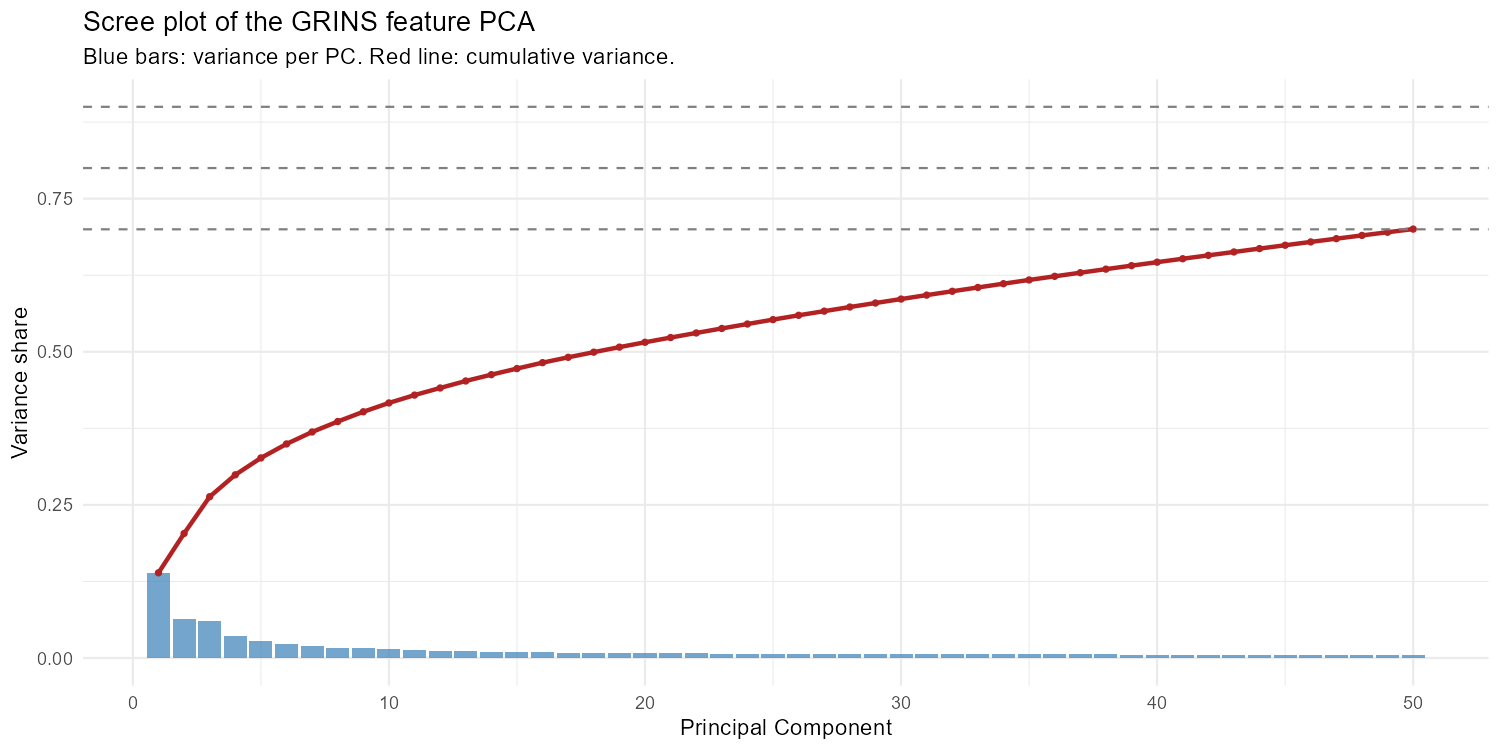
\includegraphics[width=0.85\textwidth]{figures/scree_grins.png}
  \caption{Scree plot of the PCA on the engineered GRINS V3
    matrix (first 50 PCs). Blue bars: marginal variance per PC.
    Red line: cumulative variance.}
  \label{fig:scree_grins}
\end{figure}

Table~\ref{tab:pcr_grins} and Figure~\ref{fig:trade_grins} report
the out-of-sample \(R^{2}\) of PCR as a function of \(K\). The
horizontal dashed lines mark the LASSO benchmark
(\(R^{2} = 0.825\)) and the parsimonious linear model
(\(R^{2} = 0.784\)).

\begin{table}[h!]
  \centering
  \begin{tabular}{ccccc}
    \toprule
    \(K\) & \(R^{2}\) & RMSE & MAE & cumulative variance \\
    \midrule
    5    & 0.69 (approx.) & 2.32 & 1.77 & 12\,\% \\
    25   & 0.771 & 2.00 & 1.50 & 28\,\% \\
    50   & 0.778 & 1.96 & 1.48 & 41\,\% \\
    75   & 0.779 & 1.96 & 1.47 & 50\,\% \\
    100  & \textbf{0.787} & \textbf{1.92} & \textbf{1.45} & 59\,\% \\
    \bottomrule
  \end{tabular}
  \caption{PCR on the 326-feature GRINS matrix, panel-aware 5-fold
    CV. Even with one hundred principal components, PCR remains
    below the parsimonious linear model (which uses only 25
    original variables) and four points of \(R^{2}\) below the
    LASSO benchmark.}
  \label{tab:pcr_grins}
\end{table}

\begin{figure}[h!]
  \centering
  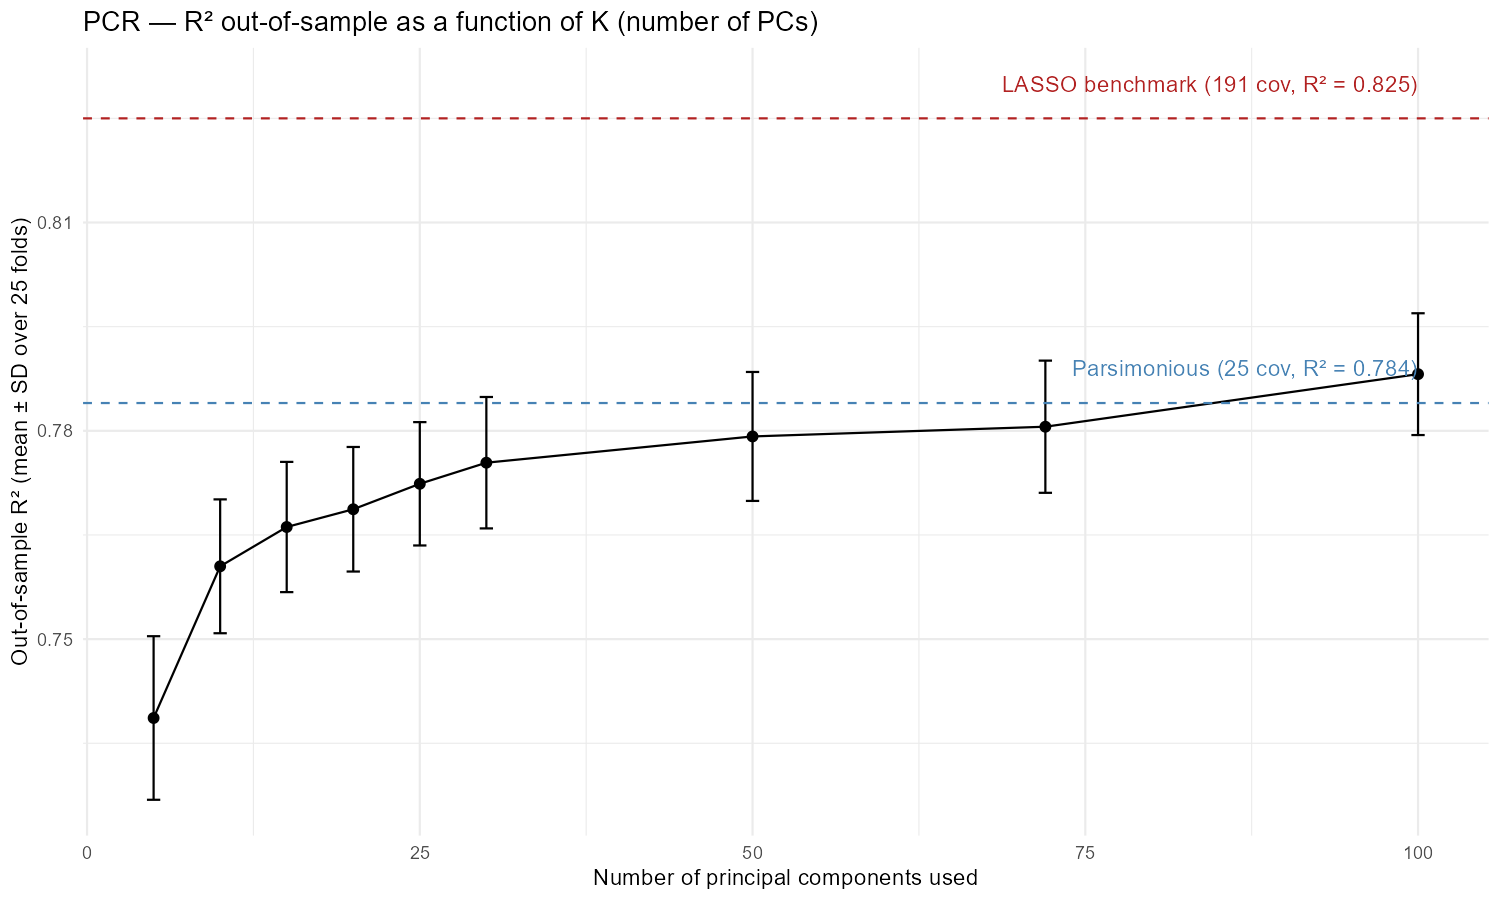
\includegraphics[width=0.85\textwidth]{figures/tradeoff_grins.png}
  \caption{PCR trade-off curve on GRINS V3 features. Mean
    out-of-sample \(R^{2}\) across 25 panel-aware CV folds, with
    \(\pm 1\) standard-deviation error bars. PCR needs about 100
    PCs to reach \(R^{2} \approx 0.787\), still below the
    parsimonious LM (25 variables, \(R^{2} = 0.784\)) and four
    points below the LASSO benchmark (191 variables,
    \(R^{2} = 0.825\)).}
  \label{fig:trade_grins}
\end{figure}

\paragraph{Two readings of the same plot.}
First, on an absolute basis, PCR cannot match the LASSO benchmark
even with five times as many components: 100 PCs achieve
\(0.787\), still \(-0.038\) below LASSO at \(0.825\). Second, on a
\emph{per-component} basis, PCR is even less efficient than the
naïve count suggests. At \(K = 25\) PCR scores \(0.772\), about
\(1.3\) percentage points below the parsimonious linear model on
the same number of original variables. This is the empirical
signature of the \emph{variance-vs-prediction misalignment}: the
principal directions of \(\mathbf{X}\) do not happen to be the
directions in which the IFC signal lives.

\subsection{PCR on the 12 IFC indicators: an almost-tautological sanity check}

The cascade scripts \texttt{02\_pca.R / 02b / 02c} compute the
descriptive PCA on the 12 IFC indicators
\(\mathrm{Ind1},\dots,\mathrm{Ind12}\). The natural predictive
counterpart is to regress the raw IFC on the leading PCs of those
same twelve indicators. Because the IFC is constructed, at least
nominally, by an aggregation of those very twelve variables, the
exercise is close to tautology: a regression on all twelve original
indicators should reproduce the IFC almost exactly.

\paragraph{A data-quality finding.}
The first run of this script returned an apparently incomplete
\(R^{2} = 0.982\). On investigation we found that the file
\texttt{IFC\_Final\_Analysis\_Sorted.xlsx} contains a small number
of duplicated \(\mathrm{PRO\_COM} \times \mathrm{year}\) entries
with inconsistent IFC values (e.g.\ municipality 5122 in 2021
appears twice with IFC = 100 and IFC = 110 respectively). The
GRINS-based pipeline masks the issue implicitly via an inner join
with a unique GRINS panel; here, with only the 12 indicators on
the predictor side, the duplicates surface. We added a
\verb|distinct(PRO_COM, year)| step to both sides of the merge
before re-running.

\paragraph{The remaining \(1.3\%\) is informative.}
After deduplication PCR with \(K = 12\) reaches
\(R^{2} = 0.987\), see Table~\ref{tab:pcr_ifc} and
Figure~\ref{fig:trade_ifc}. The residual \(1.3\%\) is small but
not zero and does not disappear with more components. It tells us
that the raw IFC is not a pure linear combination of the 12
indicators: there is a non-linear step (percentile rank,
year-specific normalisation, or similar) that the official IFC
methodology applies before the weighted aggregation. The PCR
exercise therefore doubles as a diagnostic for the IFC
construction itself.

\begin{table}[h!]
  \centering
  \begin{tabular}{cccc}
    \toprule
    \(K\) & \(R^{2}\) & cumulative variance & marginal gain \\
    \midrule
    1  & 0.648 & 29.5\,\% & --- \\
    2  & 0.741 & 43.4\,\% & \(+0.093\) \\
    3  & 0.746 & 52.2\,\% & \(+0.005\) \\
    4  & 0.763 & 60.1\,\% & \(+0.017\) \\
    \textbf{5}  & \textbf{0.899} & 67.1\,\% & \(+\mathbf{0.136}\) \\
    6  & 0.914 & 74.0\,\% & \(+0.015\) \\
    7  & 0.920 & 80.5\,\% & \(+0.006\) \\
    8  & 0.932 & 85.9\,\% & \(+0.013\) \\
    9  & 0.936 & 90.6\,\% & \(+0.003\) \\
    \textbf{10} & \textbf{0.970} & 94.6\,\% & \(+\mathbf{0.034}\) \\
    11 & 0.980 & 97.9\,\% & \(+0.010\) \\
    12 & 0.987 & 100\,\%  & \(+0.007\) \\
    \bottomrule
  \end{tabular}
  \caption{PCR on the 12 IFC indicators, panel-aware 5-fold CV
    after deduplication. The \(R^{2}\) gains are spectacularly
    \emph{non-monotone}: PC5 alone is worth more than PC1--PC4
    together, and PC10 alone is worth more than PC6--PC9 together.}
  \label{tab:pcr_ifc}
\end{table}

\begin{figure}[h!]
  \centering
  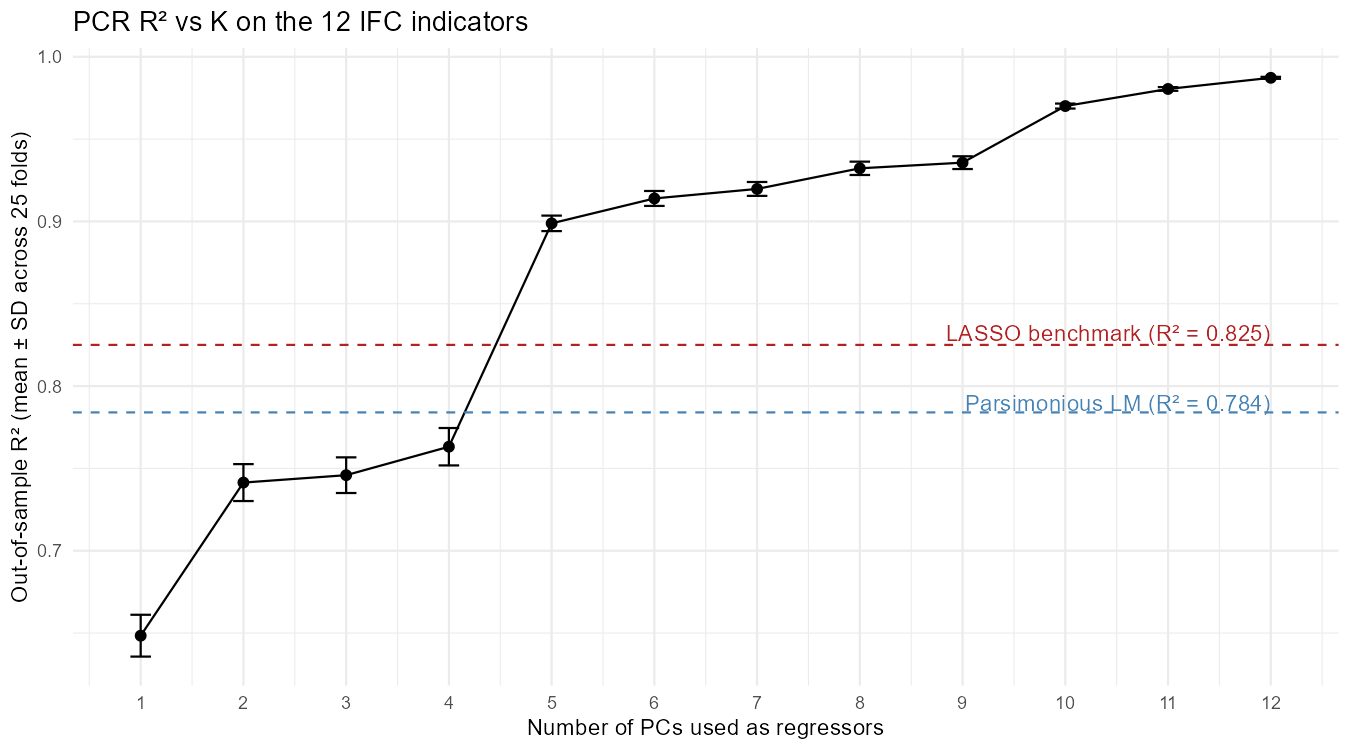
\includegraphics[width=0.85\textwidth]{figures/tradeoff_ifc.png}
  \caption{PCR trade-off curve on the 12 IFC indicators. The two
    visible jumps, between \(K = 4\) and \(K = 5\) and between
    \(K = 9\) and \(K = 10\), are the empirical signature of
    PCR's main weakness: the predictive direction does not align
    with the principal directions, so some "minor" PCs carry
    disproportionate share of the predictive content for IFC.}
  \label{fig:trade_ifc}
\end{figure}

\paragraph{A clean illustration of why PCR misranks the components.}
At \(K = 4\) PCR has used \(60\%\) of the variance of
\(\mathbf{X}\) but only achieves \(R^{2} = 0.763\). Adding PC5
brings only \(+7\%\) of variance but \(+0.14\) of \(R^{2}\). The
fifth principal direction is therefore much more informative for
the IFC than its variance share would suggest. The same is true
for PC10, with a similar discontinuity. This is the practical
reason why PLS, which uses \(y\) to order its components, is the
correct method for this kind of problem.

\subsection{Head-to-head: PLS dominates PCR}

Script 18c runs PCR and PLS on the same 326-feature GRINS matrix
and at the same set of \(K\) values. Table~\ref{tab:plspcr} and
Figure~\ref{fig:plspcr} report the result.

\begin{table}[h!]
  \centering
  \begin{tabular}{ccc c}
    \toprule
    \(K\) & PCR \(R^{2}\) & PLS \(R^{2}\) & gap PLS \(-\) PCR \\
    \midrule
    5    & 0.739 & 0.796 & \(+0.058\) \\
    10   & 0.761 & 0.810 & \(+0.049\) \\
    15   & 0.766 & 0.817 & \(+0.051\) \\
    20   & 0.769 & 0.820 & \(+0.051\) \\
    25   & 0.772 & \textbf{0.822} & \(+0.050\) \\
    30   & 0.776 & 0.823 & \(+0.047\) \\
    50   & 0.779 & 0.824 & \(+0.045\) \\
    75   & 0.780 & \textbf{0.825} & \(+0.045\) \\
    100  & 0.787 & 0.824 & \(+0.037\) \\
    \bottomrule
  \end{tabular}
  \caption{PCR vs PLS on the 326-feature GRINS matrix, panel-aware
    5-fold CV. PLS dominates PCR by approximately five points of
    \(R^{2}\) at every \(K\). PLS at \(K = 25\) already beats both
    the parsimonious linear model and the mixed-model extension;
    PLS at \(K = 75\) matches the LASSO benchmark.}
  \label{tab:plspcr}
\end{table}

\begin{figure}[h!]
  \centering
  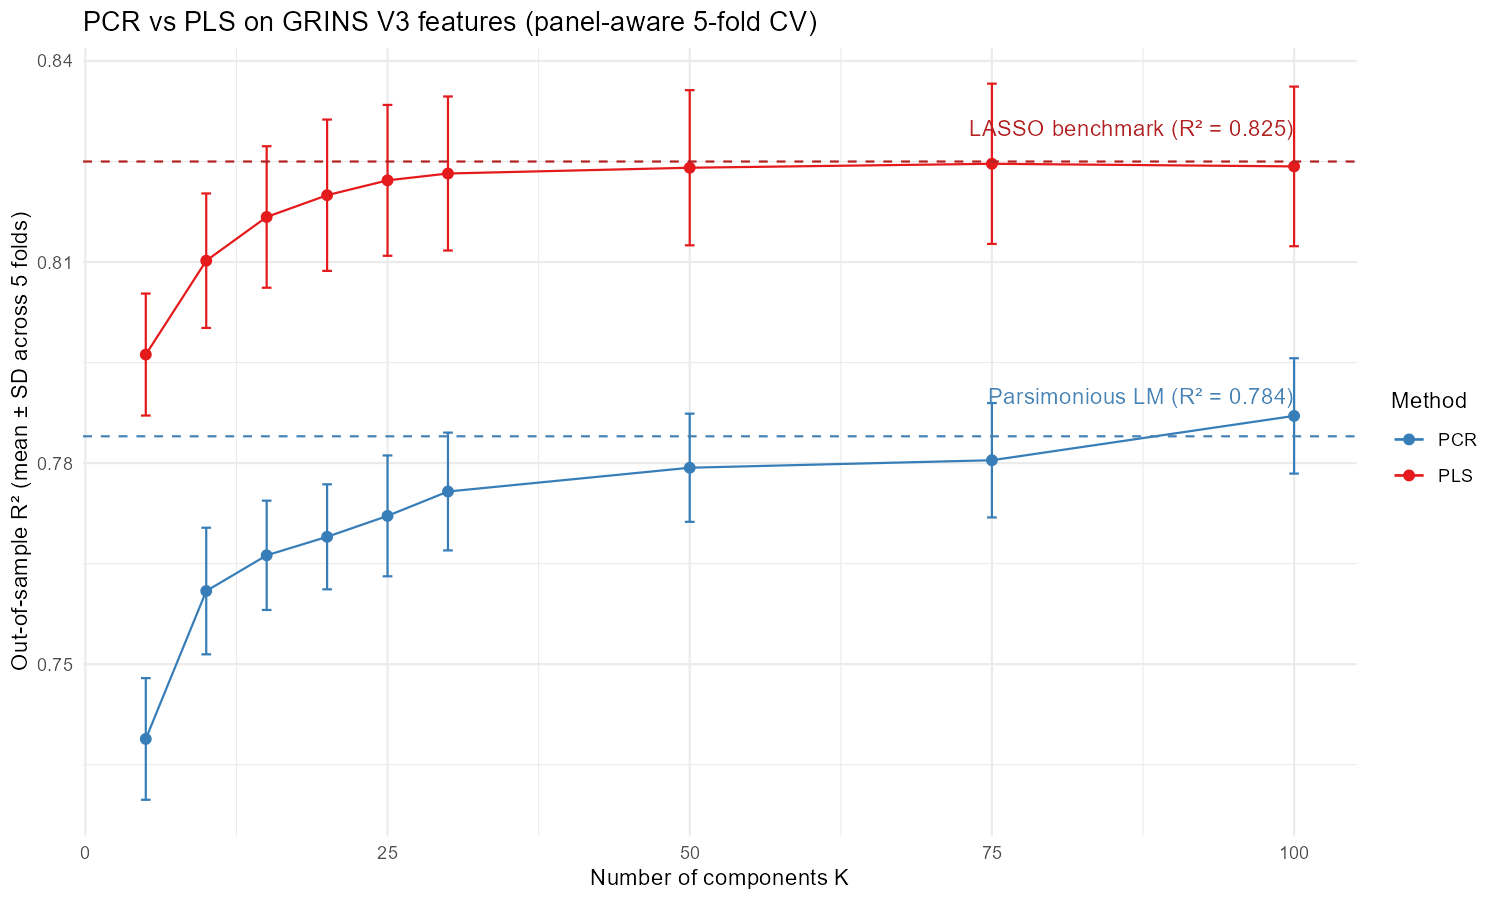
\includegraphics[width=0.95\textwidth]{figures/pls_vs_pcr.png}
  \caption{PLS vs PCR on GRINS V3 features. Out-of-sample \(R^{2}\)
    over 5 panel-aware CV folds, mean \(\pm 1\) standard
    deviation. The red dashed line is the LASSO benchmark; the
    blue dashed line is the parsimonious linear model. PLS
    reaches the LASSO benchmark at \(K \approx 75\); PCR never
    reaches it within the range explored.}
  \label{fig:plspcr}
\end{figure}

\paragraph{Three observations.}
First, the PLS--PCR gap is stable and substantial: about five
percentage points of \(R^{2}\) over the whole range of \(K\). This
is much larger than the cross-fold standard deviation
(\(\sim 0.01\)) and therefore not the artefact of one favourable
split. Second, PLS at \(K = 25\) already scores \(0.822\), which
is better than both the parsimonious linear model on the same
nominal complexity (25 dimensions) and the \(M_{\mathrm{geo,
nested}}\) mixed-model extension. PLS in this sense is a
non-interpretable upper bound on the linear-model class. Third,
PLS plateaus around \(K = 75\) at \(0.825\), essentially tied with
the LASSO benchmark at 191 covariates. The two methods reach the
same predictive ceiling by different routes: LASSO selects, PLS
combines.

\section{Comparison with the rest of the project}

Table~\ref{tab:all} aggregates all the models that have been
estimated so far. PLS at \(K=25\) and \(M_{\mathrm{geo,nested}}\)
LMM at 25 covariates are essentially tied, and only marginally
below the LASSO benchmark and PLS at \(K=75\). PCR is consistently
below this set.

\begin{table}[h!]
  \centering
  \begin{tabular}{l c c l}
    \toprule
    Model & dimensions & CV \(R^{2}\) & interpretability \\
    \midrule
    LASSO benchmark              & 191 GRINS var.  & 0.826 & high (named variables) \\
    PLS on GRINS \((K = 75)\)    & 75 components   & 0.825 & low (mixture variables) \\
    PLS on GRINS \((K = 25)\)    & 25 components   & 0.822 & low \\
    \(M_{\mathrm{geo,nested}}\) LMM & 25 var.\ + RE & 0.818 & high \\
    PCR on GRINS \((K = 100)\)   & 100 components  & 0.787 & low \\
    Parsimonious LM              & 25 GRINS var.   & 0.784 & high \\
    PCR on GRINS \((K = 25)\)    & 25 components   & 0.772 & low \\
    PCR on 12 IFC \((K = 12)\)   & 12 components   & 0.987 & near-tautological \\
    \bottomrule
  \end{tabular}
  \caption{All models considered in the project so far, sorted by
    out-of-sample \(R^{2}\) within the GRINS-based group. The
    final row is included for the diagnostic interpretation only
    (PCR on the IFC's own input indicators).}
  \label{tab:all}
\end{table}

\section{Conclusions}

The instructor's request to extend the descriptive PCA into a
Principal Component Regression has produced a coherent set of
methodological findings.

\paragraph{PCR underperforms because variance and prediction do not align.}
On both the 326-feature GRINS matrix and the 12-indicator IFC
matrix, PCR needs to use components much further down the ranking
than the principal directions to capture the IFC signal. The clearest
example is the \(+0.14\) \(R^{2}\) jump at \(K = 5\) in
Figure~\ref{fig:trade_ifc}: PC5 carries 7\% of the variance of
\(\mathbf{X}\) but more predictive content than PC1 through PC4
combined.

\paragraph{Tautology test confirms IFC is not pure-linear.}
The PCR on the 12 IFC indicators stops at \(R^{2} = 0.987\), not
at \(1.0\). The remaining \(1.3\%\) is not noise but a structural
non-linearity in the IFC construction (a percentile-rank or
similar normalisation step). This is a useful sanity check on the
target itself.

\paragraph{PLS fixes the misalignment but loses interpretability.}
PLS, which uses \(y\) in the choice of components, dominates PCR
by about five points of \(R^{2}\) at every \(K\). PLS at
\(K = 75\) matches the LASSO benchmark; PLS at \(K = 25\) is
essentially tied with the geographically nested mixed model. The
LASSO benchmark is therefore not a special accident of the
penalty: any well-chosen 75-dimensional linear projection of the
GRINS features reaches the same predictive ceiling. What LASSO
buys is \emph{interpretability}: 25 named covariates with
explicit signs and standardised effects, instead of 25 or 75
linear combinations of all 326 features.

\paragraph{Take-away for the project.}
The LASSO + LMM pipeline retains its place as the preferred
deliverable. PCR is documented here as a methodological control
(it is what one obtains by treating dimensionality reduction as a
substitute for variable selection), and PLS is documented as the
best linear non-interpretable upper bound. The choice between
LASSO and PLS at \(K = 75\) is essentially a choice between
interpretable variables and an unreadable but slightly larger
model: in our setting they reach the same predictive accuracy.

\end{document}
